\documentclass[english,,man]{apa6}
\usepackage{lmodern}
\usepackage{amssymb,amsmath}
\usepackage{ifxetex,ifluatex}
\usepackage{fixltx2e} % provides \textsubscript
\ifnum 0\ifxetex 1\fi\ifluatex 1\fi=0 % if pdftex
  \usepackage[T1]{fontenc}
  \usepackage[utf8]{inputenc}
\else % if luatex or xelatex
  \ifxetex
    \usepackage{mathspec}
  \else
    \usepackage{fontspec}
  \fi
  \defaultfontfeatures{Ligatures=TeX,Scale=MatchLowercase}
\fi
% use upquote if available, for straight quotes in verbatim environments
\IfFileExists{upquote.sty}{\usepackage{upquote}}{}
% use microtype if available
\IfFileExists{microtype.sty}{%
\usepackage{microtype}
\UseMicrotypeSet[protrusion]{basicmath} % disable protrusion for tt fonts
}{}
\usepackage{hyperref}
\hypersetup{unicode=true,
            pdftitle={Process Cookbook},
            pdfauthor={\ldots{}},
            pdfkeywords={\ldots{}.},
            pdfborder={0 0 0},
            breaklinks=true}
\urlstyle{same}  % don't use monospace font for urls
\ifnum 0\ifxetex 1\fi\ifluatex 1\fi=0 % if pdftex
  \usepackage[shorthands=off,main=english]{babel}
\else
  \usepackage{polyglossia}
  \setmainlanguage[]{english}
\fi
\usepackage{graphicx,grffile}
\makeatletter
\def\maxwidth{\ifdim\Gin@nat@width>\linewidth\linewidth\else\Gin@nat@width\fi}
\def\maxheight{\ifdim\Gin@nat@height>\textheight\textheight\else\Gin@nat@height\fi}
\makeatother
% Scale images if necessary, so that they will not overflow the page
% margins by default, and it is still possible to overwrite the defaults
% using explicit options in \includegraphics[width, height, ...]{}
\setkeys{Gin}{width=\maxwidth,height=\maxheight,keepaspectratio}
\IfFileExists{parskip.sty}{%
\usepackage{parskip}
}{% else
\setlength{\parindent}{0pt}
\setlength{\parskip}{6pt plus 2pt minus 1pt}
}
\setlength{\emergencystretch}{3em}  % prevent overfull lines
\providecommand{\tightlist}{%
  \setlength{\itemsep}{0pt}\setlength{\parskip}{0pt}}
\setcounter{secnumdepth}{0}
% Redefines (sub)paragraphs to behave more like sections
\ifx\paragraph\undefined\else
\let\oldparagraph\paragraph
\renewcommand{\paragraph}[1]{\oldparagraph{#1}\mbox{}}
\fi
\ifx\subparagraph\undefined\else
\let\oldsubparagraph\subparagraph
\renewcommand{\subparagraph}[1]{\oldsubparagraph{#1}\mbox{}}
\fi

%%% Use protect on footnotes to avoid problems with footnotes in titles
\let\rmarkdownfootnote\footnote%
\def\footnote{\protect\rmarkdownfootnote}


  \title{Process Cookbook}
    \author{\ldots{}\textsuperscript{1}}
    \date{}
  
\shorttitle{PROCESS INFERENCES}
\authornote{....


Correspondence concerning this article should be addressed to ..., .... E-mail: ...}
\affiliation{
\vspace{0.5cm}
\textsuperscript{1} ...}
\abstract{Begin here...
}
\keywords{....\newline\indent Word count: 95}
\usepackage{csquotes}
\usepackage{upgreek}
\captionsetup{font=singlespacing,justification=justified}

\usepackage{longtable}
\usepackage{lscape}
\usepackage{multirow}
\usepackage{tabularx}
\usepackage[flushleft]{threeparttable}
\usepackage{threeparttablex}

\newenvironment{lltable}{\begin{landscape}\begin{center}\begin{ThreePartTable}}{\end{ThreePartTable}\end{center}\end{landscape}}

\makeatletter
\newcommand\LastLTentrywidth{1em}
\newlength\longtablewidth
\setlength{\longtablewidth}{1in}
\newcommand{\getlongtablewidth}{\begingroup \ifcsname LT@\roman{LT@tables}\endcsname \global\longtablewidth=0pt \renewcommand{\LT@entry}[2]{\global\advance\longtablewidth by ##2\relax\gdef\LastLTentrywidth{##2}}\@nameuse{LT@\roman{LT@tables}} \fi \endgroup}


\DeclareDelayedFloatFlavor{ThreePartTable}{table}
\DeclareDelayedFloatFlavor{lltable}{table}
\DeclareDelayedFloatFlavor*{longtable}{table}
\makeatletter
\renewcommand{\efloat@iwrite}[1]{\immediate\expandafter\protected@write\csname efloat@post#1\endcsname{}}
\makeatother
\usepackage{lineno}

\linenumbers

\usepackage{amsthm}
\newtheorem{theorem}{Theorem}[section]
\newtheorem{lemma}{Lemma}[section]
\theoremstyle{definition}
\newtheorem{definition}{Definition}[section]
\newtheorem{corollary}{Corollary}[section]
\newtheorem{proposition}{Proposition}[section]
\theoremstyle{definition}
\newtheorem{example}{Example}[section]
\theoremstyle{definition}
\newtheorem{exercise}{Exercise}[section]
\theoremstyle{remark}
\newtheorem*{remark}{Remark}
\newtheorem*{solution}{Solution}
\begin{document}
\maketitle

Take aways from last time:

\begin{itemize}
\item
  Change hook

  \begin{itemize}
  \tightlist
  \item
    Not a \enquote{this is what true process is} paper. An organizing
    paper on the inferences people make and the models they use with
    longitudinal data.
  \end{itemize}
\item
  Change structure

  \begin{itemize}
  \item
    Start early with Xu and DeShon figure to organize everything
  \item
    Use generic variables throughout
  \item
    Data structures issues at end
  \end{itemize}
\end{itemize}

\hypertarget{hook}{%
\section{Hook}\label{hook}}

The story:

\begin{itemize}
\tightlist
\item
  People want us to do stuff with longitudinal data, to make inferences
  over time. But this literature can be confusing. We could use some
  organization.
\end{itemize}

New researchers are increasingly asked to collect longitudinal data and
study how things happen over time. They are advised to because the
organizational and psychological processes we study \enquote{are not
static but instead develop, change, and evolve over time} (Pitariu \&
Ployhart, p.~405) and \enquote{many, if not most, of the psychological
phenomena in which we are interested are\ldots{}sequences of events and
event reactions that play out within each person's stream of experience}
(Beal, 2015, p.~5). If a researcher can collect longitudinal data, they
are then in a better position to understand patterns over time. Bell and
Kozlowski (2003), for example, state that \enquote{longitudinal
designs\ldots{}will be far more revealing of the team phenomeon under
investigation} (p.~59). Similarly -- in their review of emotional labor
-- Grandey and Gabriel (2015) suggest that future researchers may be
much better equipped to demonstrate emotion regulation patters
\enquote{with longitudinal methods} (p.~329). Not only do longitudinal
data collections help the researcher observe relationships over time,
many argue that it helps refine and strengthen our theories. For
instance, Pitariu and Ployhart (2010) suggest that collecting
longitudinal data, observing change, and testing dynamic models
\enquote{stimulates greater refinement in our existing theories}
(p.~411), and Grandey and Gabriel (2015) urge for greater theoretical
development of emotions by studying their \enquote{reciprocal and
unfolding\ldots{}processes\ldots{}through momentary assessments or
lagged effects} (p.~322). These quotes reveal our field's emphasis on
collecting longitudinal data to sufficiently observe a process and build
better theory -- and suggest to newcomers that their designs ought to
entail repeated assessments.

To satisfy these calls, a newcomer might look to our existing literature
for examples of how others understand the patterns they observe in
longitudinal designs; this literature is not hard to find. Empirical
studies commonly employ repeated measures and the number of time points
they use appears to be growing. Words such as \enquote{dynamic,}
\enquote{change}, and \enquote{process} are becoming more prevalent in
our literature. Event-sampling methods, which collect repeated
observations by necessity, are becomming one of the most popular data
collection techniques (Beal, 2015). Finally, a quick skim over the
latest issues of top organizational journals reveals that many new
studies employ longitudinal designs.

Although our researcher would find some similarities across this
literature, she would be confronted by many more areas of disconnect.
Some studies use hierarchical linear models (HLM), whereas others employ
latent growth curves -- even when the underlying questions that they
examine are the same. Some make inferences about change, whereas others
are interested in dynamics or growth -- even when the models they apply
are identical. Some propose hypotheses with lags, whereas others do not
-- even when both collect data across the same number of time points and
interval spacing. All of these authors examine patterns in longitudinal
data, but it can be unclear how they fit together across their seemingly
unrelated hypotheses, models, and inferences. What, then, is a new
researcher interested in making inferences with respect to their
longitudinal data to do?

Our goal is to organize the common inferences made with longitudinal
data so that researchers have a clear sense of what hypotheses they can
propose, models they can use, and inferences they can make given their
data structure and research question. Our literature is starting to
accumulate great examples of the types of inferences we can make with
longitudinal data, but their similarities and strengths can sometimes go
unnoticed due to the different language used by separate content and
statistical modeling areas. Two studies may be interested in the same
type of question or inference but apply different models to their data
or describe their results with dissimilar variable names. Rather than
miss the common ground between these two, we want to provide a framework
for seeing how both provide similar types of knowledge. On the other
hand, just because two researchers study something over time does not
mean they provide the same type of information -- and we want to help
researchers avoid misconstrued similarities. Moreover, there are small
differences in how we conceptualize and model longitudinal data that
result in vastly different inferences. In this paper, therefore, we want
to organize the inferences researchers make with longitudinal data.

Below, we discuss four common longitudinal research areas: relationships
over time, growth, change, and dynamics. These do not represent every
possible domain we can explore with longitudinal data, but they do cover
a large portion of the techniques currently employed in our literature.
We begin by explaining what we mean by longitudinal research. We then
unpack a framework proposed by Xu and DeShon that relates the four
different research streams. In the core of the paper, we discuss each
stream in depth, provide examples from the literature, point researchers
to potential models, and acknowledge the pitfall and limitations of each
approach.

\hypertarget{intro}{%
\section{Intro}\label{intro}}

\textbf{Define longitudinal}

This paper is exclusively devoted to the inferences we make with
repeated observations, so we begin by identifying a few labels and
definitions. Authors typically identify a \enquote{longitudinal} study
by making a contrast with respect to either a) research designs or b)
data structures. Longitudinal \emph{research} is different from
cross-sectional research because longitudinal designs entail three or
more repeated observations (Ployhart \& Bliese, Singer \& Willett). We
therefore emphasize differences on the number of observations when we
distinguish longitudinal from other types of research. Longitudinal
\emph{data} are repeated observations on several units (i.e., \(N\) or
\(i\) \textgreater{} 1), whereas panel data are a collection of
observations of one unit over time -- a distinction that focuses on the
amount of people in our study. Most organizational studies collect data
on more than one unit, therefore our discussion below focuses on
longitudinal research with longitudinal data, or designs with \(N\)
\textgreater{} 1, \(t\) \textgreater{}= 3, and the same construct(s)
measured on each \(i\) at each \(t\).

\textbf{Introduce framework}

Presenting the entire inference and modeling literature that uses
longitudinal data structures would be impossible. Instead, we focus on
four related streams that we feel can be organized nicely using a
framework proposed by Xu and DeShon. Figure one shows each inference we
will discuss in this paper: relationships, growth, change, and dynamics.

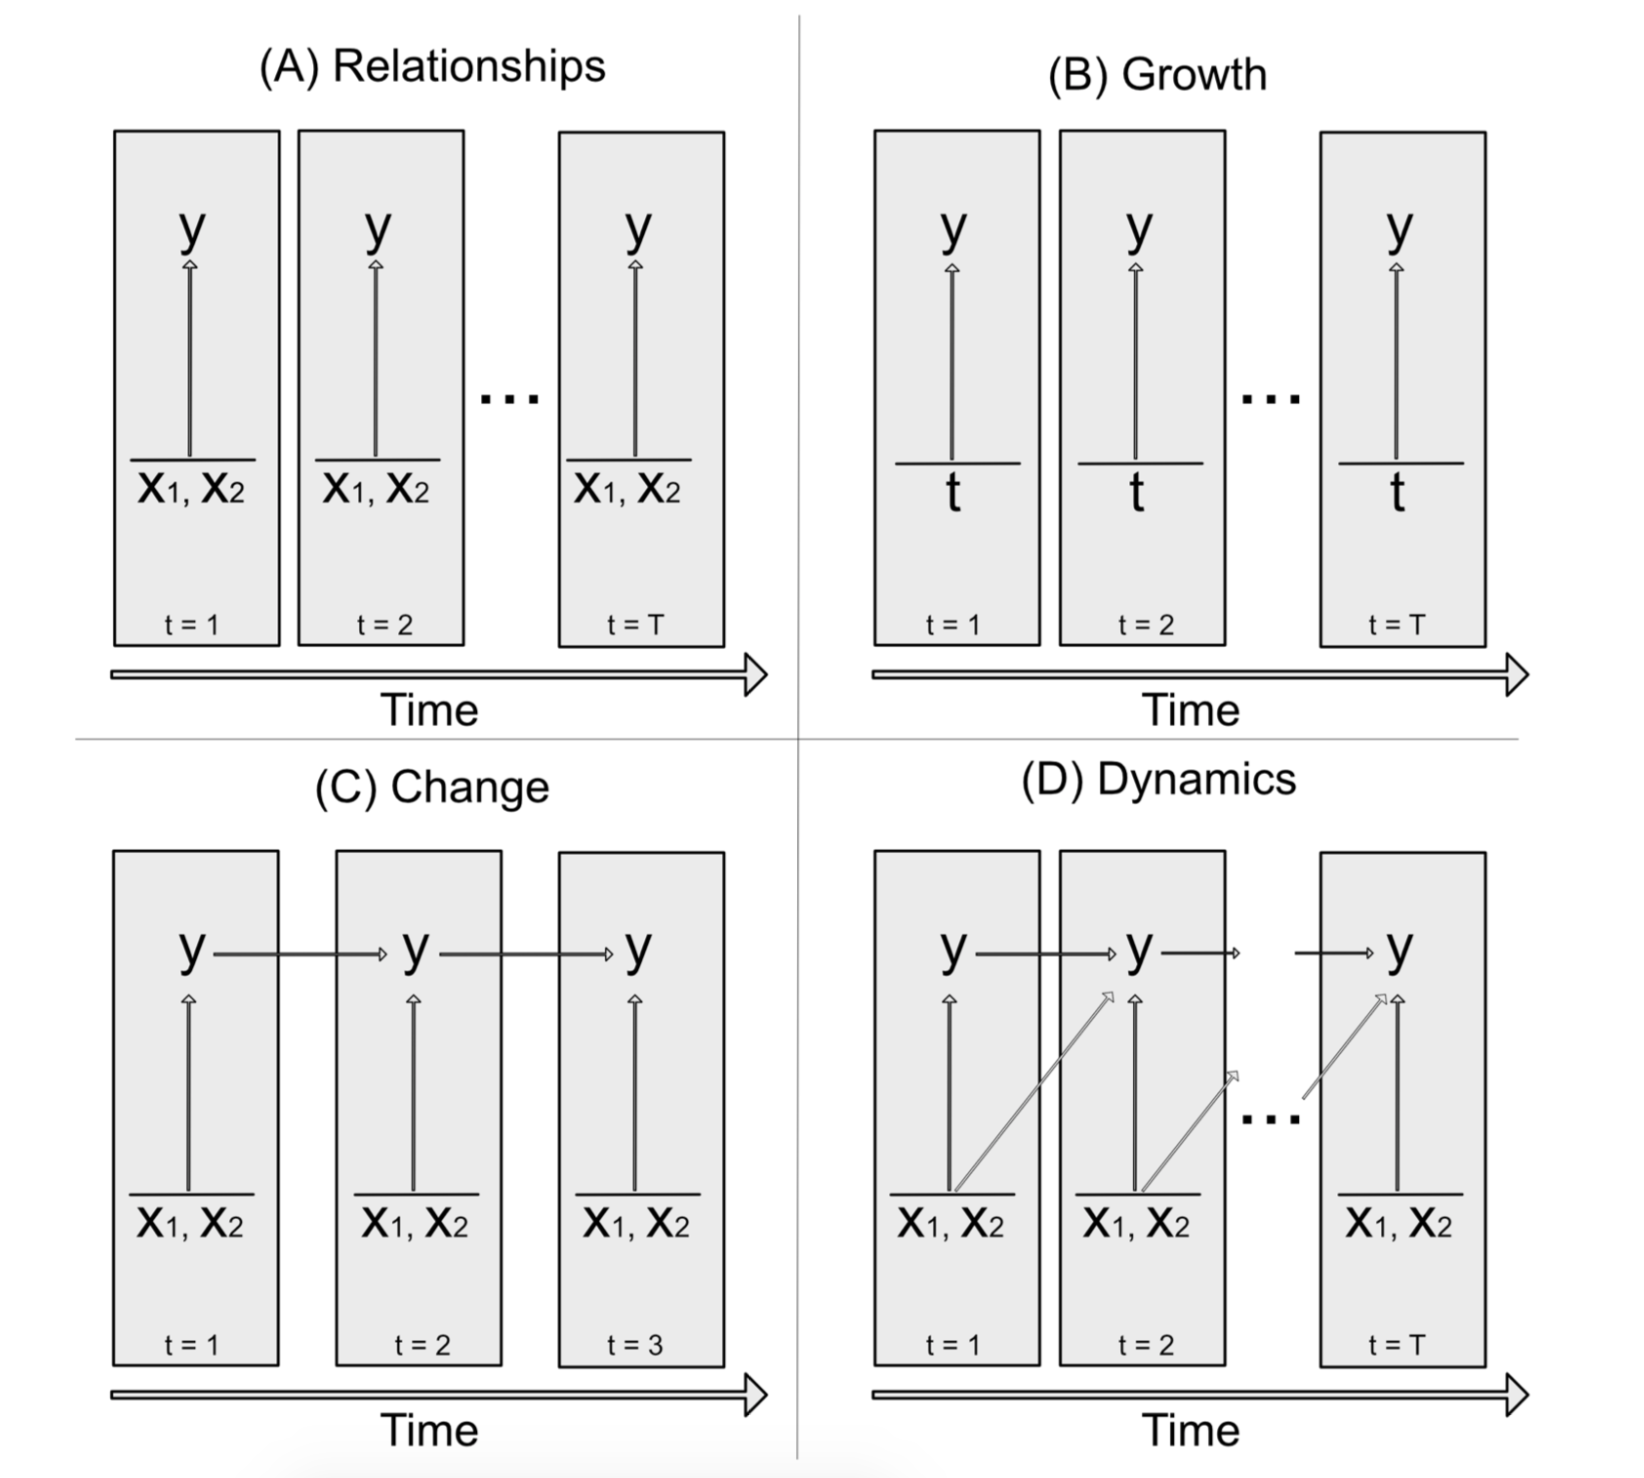
\includegraphics{figures/common_models.png}

\textbf{Discuss each briefly}

\textbf{Provide generic variable names to use throughout}

\textbf{Examples}

\hypertarget{relationships-goran-mike-rick-do-not-read-past-here-this-is-the-same-as-last-timenot-updated-yet}{%
\section{Relationships (Goran, Mike, Rick do not read past here, this is
the same as last time\ldots{}not updated
yet)}\label{relationships-goran-mike-rick-do-not-read-past-here-this-is-the-same-as-last-timenot-updated-yet}}

\hypertarget{inference-1}{%
\subsection{Inference 1}\label{inference-1}}

The relationship of one or more predictor variables with a response
variable over time.

\hypertarget{examples}{%
\subsubsection{Examples}\label{examples}}

\hypertarget{hypotheses}{%
\paragraph{Hypotheses}\label{hypotheses}}

Barnes, Schaubroeck, Huth, and Ghumman (2011) and Chi, Chang, and Huang
(2015) present hypotheses that are consistent with a relationships
inference. Barnes et al. (2011) predict a negative relationship between
poor sleep and cognitive self control. Similarly, Chi et al. (2015)
hypothesize that daily negative mood negatively relates to daily task
performance.

\hypertarget{longitudinal-data-structure}{%
\paragraph{Longitudinal Data
Structure}\label{longitudinal-data-structure}}

Researchers that infer relationships over time either a) measure their
variables at the same time points or b) treat the data as if they were
measured as so by the constraints of their analysis. Barnes et al.
(2011) give an example of the former; they measure sleep and cognitive
self control every morning for five consecutive days (study 4). Chi et
al. (2015), as an example of the latter, measure negative mood in the
morning and task performance in the afternoon -- but these variables are
treated as if they were taken at the same time (e.g., day 4) when
entered into their analysis (described later).

There is no limit to the number of possible time points, but studies of
this type typically collect between three and ten repeated measurements.
Our examples above measure their variables once per day, but other
frequencies could also be used. Methods literature typically recommends
that researchers maintain the same interval between each measurement
across their study, but this can be difficult when studies last longer
than a week. For example, Chi et al. (2015) take their measurements for
ten work days. In the middle of those assessments, however, their sample
employees go home for the weekend and are not measured. The space,
therefore, between \(t\) and \(t + 1\) is not the same across their
analysis. Finally, our organizational literature almost always takes
measures on more than one unit across time.

\hypertarget{models}{%
\paragraph{Models}\label{models}}

Both Barnes et al. (2011) and Chi et al. (2015) use hiearchical linear
modeling (HLM) -- also known as multi-level or random coefficient models
-- to estimate the parameters that generate their observed data. Random
coefficient models assume that their random effects are distributed
\(N(\gamma, \sigma^2)\) -- but this statement is easier to understand
with a contrast. Imagine that everyone in the sample receives their own
\(X_t\) on \(Y_t\) effect and we then summarize those effects by taking
their average. HLM, conversely, estimates one \(X_t\) on \(Y_t\) effect
across units (people) but does so by imposing a normality constraint.
Finally, Barnes et al. (2011) and Chi et al. (2015) use models that fall
into the broader time-varying analysis class because their measurements
of \(X\) are allowed to vary over time. In time-invariant analyses,
conversely, values of the covariate remain stable (e.g., gender).

\hypertarget{pitfalls-and-recommendations}{%
\subsubsection{Pitfalls and
Recommendations}\label{pitfalls-and-recommendations}}

What can go wrong. Recommendation. Why.

\hypertarget{growth}{%
\section{Growth}\label{growth}}

\hypertarget{inference-1-1}{%
\subsection{Inference 1}\label{inference-1-1}}

What is the level of a construct at a given point in time?

\hypertarget{examples-1}{%
\subsubsection{Examples}\label{examples-1}}

\hypertarget{hypotheses-1}{%
\paragraph{Hypotheses}\label{hypotheses-1}}

There are few (if any) studies that make direct predictions about
construct levels at certain time points. Almost every longitudinal
study, however, estimates an intercept term to approximate the answer.
These terms are then discussed in the context of broader growth
inferences that we discuss below.

\hypertarget{longitudinal-data-structure-1}{%
\paragraph{Longitudinal Data
Structure}\label{longitudinal-data-structure-1}}

This inference requires several repeated measures on one variable. For
example, Zhu, Wanberg, Harrison, and Diehn (2016) measure work
adjustment once a month for nine months (among expatriates) and Jones et
al. (2016) measure concealing behaviors (among pregnant women) every
week -- but it is not clear for how long they do so.

\hypertarget{models-1}{%
\paragraph{Models}\label{models-1}}

Zhu et al. (2016) use HLM to estimate their parmaters, whereas Jones et
al. (2016) do so in a structural equation modeling framework. As stated,
researchers are interested in an intercept estimate for this inference,
and although they can place it on any time point, researchers typically
use their first observation. In SEM, the intercept is a latent variable
regressed on either an observed indicator (again, usually the first
observation) or its latent equivalent. Jones et al. (2016), for example,
regress their latent concealing behaviors intercept term on the latent
variable for concealing behaviors at time one. In HLM, the investigator
first creates a variable that represents time and then regresses the
outcome on this time indicator to estimate an intercept term. For
example, Zhu et al. (2016) regress work adjustment on time using HLM to
estimate its initial level.

\hypertarget{pitfalls-and-recommendations-1}{%
\subsubsection{Pitfalls and
Recommendations}\label{pitfalls-and-recommendations-1}}

What can go wrong. Recommendations. Why.

\hypertarget{inference-2}{%
\subsection{Inference 2}\label{inference-2}}

What are the patterns of a trajectory or trajectories across time? How
does the construct change over time?

\hypertarget{examples-2}{%
\subsubsection{Examples}\label{examples-2}}

\hypertarget{hypotheses-2}{%
\paragraph{Hypotheses}\label{hypotheses-2}}

Zhu et al. (2016) predict that expatriate work adjustment follows a
positive trajectory, increasing over the time of the assignment.
Similarly, Jones et al. (2016) hypothesize that concealing behaviors
will have negative slopes over time.

\hypertarget{longitudinal-data-structure-2}{%
\paragraph{Longitudinal Data
Structure}\label{longitudinal-data-structure-2}}

As with our previous inference, the only requirement here is a repeated
assessment on one variable over several time points -- both Zhu et al.
(2016) and Jones et al. (2016) meet these requirements.

\hypertarget{models-2}{%
\paragraph{Models}\label{models-2}}

Researchers use slope terms in their models for making inferences about
trajectory patterns. In HLM, the same procedure we described above --
regressing the outcome on time -- also provides a slope estimate.
Typically researchers do not allow their slope estimates to vary over
units, but the models can easily support random slope terms. Zhu et al.
(2016), for example, estimate a random slope effect by regressing work
adjustment on time. In SEM, a latent slope term is regressed onto all
time points except for the time point that was used by the latent
intercept term. Jones et al. (2016) regress a latent concealing
behaviors slope term on latent concealing behaviors at all time points
beyond \(t_1\).

Researchers may also be interested in curvilinear slopes. The only
additional requirement for doing so is to create other time indicators
with respect to the higher order polynomial. Zhu et al. (2016), for
example, included linear, quadratic, and cubic time variables to
estimate different slope curves. Note that these are still
\enquote{linear} processes because they are linear in parameters.

\hypertarget{pitfalls-and-recommendations-2}{%
\subsubsection{Pitfalls and
Recommendations}\label{pitfalls-and-recommendations-2}}

What can go wrong. Recommendations. Why.

\hypertarget{inference-3}{%
\subsection{Inference 3}\label{inference-3}}

Are there between person differences in trajectories or levels?

\hypertarget{examples-3}{%
\subsubsection{Examples}\label{examples-3}}

\hypertarget{hypotheses-3}{%
\paragraph{Hypotheses}\label{hypotheses-3}}

Similar to our first growth inference, researchers rarely make a direct
prediction about between person differences in trajectory or level, but
it is almost always included as part of a larger growth analysis.

\hypertarget{longitudinal-data-structure-3}{%
\paragraph{Longitudinal Data
Structure}\label{longitudinal-data-structure-3}}

We now require repeated observations on multiple units to examine
between person (unit) differences. For example, Zhu et al. (2016)
collect data from 179 expatriates across nine consecutive months.

\hypertarget{models-3}{%
\paragraph{Models}\label{models-3}}

Models that estimate intercept or slope terms also estimate a variance
on those terms, and these are then subjected to significance tests. When
the variance on the intercept is significant, that is taken to mean that
there are between unit differences in intercept (levels), whereas
significant variance estimates on the slope terms indicates between unit
differences in slope (trajectory). Zhu et al. (2016) use HLM to estimate
the variance on their intercept and slope terms and find evidence of
between person differences in work adjustment intercept (level) and
slope (trajectory).

\hypertarget{pitfalls-and-recommendations-3}{%
\subsubsection{Pitfalls and
Recommendations}\label{pitfalls-and-recommendations-3}}

What can go wrong. Recommendations. Why.

\hypertarget{inference-4}{%
\subsection{Inference 4}\label{inference-4}}

How is the level of a construct related to the trajectory of the same or
different constructs? What is the correlation between intercept and
slope terms?

\hypertarget{examples-4}{%
\subsubsection{Examples}\label{examples-4}}

\hypertarget{hypotheses-4}{%
\paragraph{Hypotheses}\label{hypotheses-4}}

Schaubroeck, Lam, and Peng (2016) predict that initial levels of peer
leader's transformational leadership will positively relate to the slope
of employee beliefs. Zhu et al. (2016) hypothesize that initial level of
expatriate work adjustment is negatively related to the speed of change
in work adjustment. Notice that the first prediction is about how the
level of one construct is related to the slope of another, whereas the
second focuses only on a single variable. Although it is uncommon in our
literature, developmental researchers will also predict associations
between slope and the final -- rather than initial -- observation.

\hypertarget{longitudinal-data-structure-4}{%
\paragraph{Longitudinal Data
Structure}\label{longitudinal-data-structure-4}}

Data structures that researchers use to examine this inference are
consistent with what we have already reviewed. Schaubroeck et al. (2016)
measured transformational leadership and employee beliefs at three time
points. Their time two assessment was 10 weeks after their first
observation, whereas their final measurement was taken 10 months after
their second observation. That is, the data structure for their
respective time points were \(t\), \(t + 10\), and \(t + 40\). As stated
above, Zhu et al. (2016) collected data once a month for nine months.

\hypertarget{models-4}{%
\paragraph{Models}\label{models-4}}

Both HLM and SEM provide estimates of the covariance between the
intercept and slope terms discussed above, and this covariance indicates
the association between level and trajectory. For example, Zhu et al.
(2016) report a negative covariance estimate betwen the initial level of
expatriate work adjustment (intercept) and its linear trajectory over
time (slope). As stated, researchers can also examine this association
but among the level of one variable and the trajectory of a different
variable. Schaubroeck et al. (2016) report an estimate of the
relationship between transformational leadership intercept and employee
beliefs slope. It is often helpful to generate predicted values using
the analysis estimates and then plot the levels and trajectories to
interpret them appropriately.

\hypertarget{pitfalls-and-recommendations-4}{%
\subsubsection{Pitfalls and
Recommendations}\label{pitfalls-and-recommendations-4}}

What can go wrong. Recommendations. Why.

\hypertarget{inference-5}{%
\subsection{Inference 5}\label{inference-5}}

What inter-individual characteristics relate to intra-individual
differences in level or slope?

\hypertarget{examples-5}{%
\subsubsection{Examples}\label{examples-5}}

\hypertarget{hypotheses-5}{%
\paragraph{Hypotheses}\label{hypotheses-5}}

Inferences of this type take the form of stable unit effects and their
relationship with trajectory or level. Li, Burch, and Lee (2017) predict
a positive relationship between job strain and job complexity
trajectory. Zhu et al. (2016) hypothesize that the trajectory of
expatriate work adjustment is positively related to perceived career
instrumentality. Finally, Jones et al. (2016) make two inferences of
this type: contextual support is a) negatively related to average levels
of concealing but b) positively related to the slope of concealing.

\hypertarget{longitudinal-data-structures}{%
\paragraph{Longitudinal Data
Structures}\label{longitudinal-data-structures}}

We discussed the data structures for Zhu et al. (2016) and Jones et al.
(2016) above. Li et al. (2017) use a similar design but their data are
collected once per year. Job complexity is measured once every year for
three years, and job strain is measured once at the final time point
(year 3).

\hypertarget{models-5}{%
\paragraph{Models}\label{models-5}}

Both Li et al. (2017) and Zhu et al. (2016) use HLM to estimate their
parameters, whereas Jones et al. (2016) do so with SEM. In these models,
the intercept or slope terms discussed above are regressed onto the
inter-individual characteristic. For example, Li et al. (2017) report
the estimate of job strain predicting job complexity trajectory and Zhu
et al. (2016) do the same but for career instrumentality and job
complexity trajectory. In the SEM framework, Jones et al. (2016) report
estimates of contextual support predicting concealing slope and
intercept. Note that these models fit into the broader time-invariant
analysis class that contrast with the time-variant covariates analyses
discussed earlier.

\hypertarget{pitfalls-and-recommendations-5}{%
\subsubsection{Pitfalls and
Recommendations}\label{pitfalls-and-recommendations-5}}

What can go wrong. Recommendations. Why.

\hypertarget{change}{%
\section{Change}\label{change}}

\hypertarget{inference-1-2}{%
\subsection{Inference 1}\label{inference-1-2}}

How are the changes of one variable associated with changes in another
over time?

\hypertarget{examples-6}{%
\subsubsection{Examples}\label{examples-6}}

\hypertarget{hypotheses-6}{%
\paragraph{Hypotheses}\label{hypotheses-6}}

Change inferences are similar to relationship inferences in that they
relate a predictor to a response at the same time point, but the
researcher now wants to know whether the predictor is associated with an
increase or decrease of the outcome. For example, Johnson, Lanaj, and
Barnes (2014) predict that, within individuals, exhibiting daily
procedural justice behavior is associated with an increase in resource
depletion. Similarly, Lanaj, Johnson, and Lee (2016) hypothesize that,
within individuals, transformational leadership is associated with a
decrease in negative affect.

\hypertarget{longitudinal-data-structures-1}{%
\paragraph{Longitudinal Data
Structures}\label{longitudinal-data-structures-1}}

Johnson et al. (2014) measured justice behavior and resource depletion
in the afternoon of 10 consecutive workdays. Lanaj et al. (2016)
measured their variables at different frequencies. They measured
transformational leadership and negative affect in the afternoon of 15
consecutive workdays, but they also took an additional measurement of
negative affect every morning -- creating a data structure of three
variables: negative affect from \(t\) to \(t + 15\), transformational
leadership from \(t\) to \(t + 15\) and morning negative affect from
\(t\) to \(t + 15\). That is, they essentially doubled the time points
of negative affect -- from \(t\) to \(t + 30\) by measuring it twice as
frequently.

\hypertarget{models-6}{%
\paragraph{Models}\label{models-6}}

Johnson et al. (2014) and Lanaj et al. (2016) employ HLM change models
that are consistent with our literature's preference for using partialed
values of the outcome variable rather than difference scores. In models
of this type, researchers regress their outcome on the predictor at the
same time point and the prior value of the outcome variable. For
example, Johnson et al. (2014) regressed resource depletion at time
\(t\) on 1) procedural justice behavior at time \(t\) and 2) resource
depletion at time \(t-1\); they then report the relationship between
justice behavior and resource depletion change. Similarly, Lanaj et al.
(2016) regress negative affect at time \(t\) on 1) transformational
leadership at time \(t\) and 2) negative affect at time \(t-1\) (i.e.,
morning negative affect) and report the association between
transformational leadership and affect change. Note that, due to the
different data sampling strategies, Johnson et al. (2014) reports change
from the prior day, whereas Lanaj et al. (2016) report change from the
morning to afternoon.

\hypertarget{pitfalls-and-recommendations-6}{%
\subsubsection{Pitfalls and
Recommendations}\label{pitfalls-and-recommendations-6}}

What can go wrong. Recommendations. Why.

\hypertarget{dynamics}{%
\section{Dynamics}\label{dynamics}}

The core concept is: how are prior states related to future states?

\hypertarget{inference-1-3}{%
\subsection{Inference 1}\label{inference-1-3}}

How is one variable related to its future self?

\hypertarget{examples-7}{%
\subsubsection{Examples}\label{examples-7}}

\hypertarget{hypotheses-7}{%
\paragraph{Hypotheses}\label{hypotheses-7}}

\hypertarget{longitudinal-data-structures-2}{%
\paragraph{Longitudinal Data
Structures}\label{longitudinal-data-structures-2}}

\hypertarget{models-7}{%
\paragraph{Models}\label{models-7}}

\hypertarget{pitfalls-and-recommendations-7}{%
\subsubsection{Pitfalls and
Recommendations}\label{pitfalls-and-recommendations-7}}

\hypertarget{inference-2-1}{%
\subsection{Inference 2}\label{inference-2-1}}

How is one variable related to a different variable in the future?

\hypertarget{examples-8}{%
\subsubsection{Examples}\label{examples-8}}

\hypertarget{hypotheses-8}{%
\paragraph{Hypotheses}\label{hypotheses-8}}

Gabriel, Diefendorff, Chandler, Moran, and Greguras (2014) hypothesize
that perceived P-O fit is positively related to subsequent positive
affect.

\hypertarget{longitudinal-data-structure-5}{%
\paragraph{Longitudinal Data
Structure}\label{longitudinal-data-structure-5}}

Gabriel et al. (2014) measured perceived P-O fit and positive affect
five times per day for 10 consecutive work days.

\hypertarget{models-8}{%
\paragraph{Models}\label{models-8}}

Researchers that use models related to this inference regress their
outcome at time \(t\) on a prior value of the independent variable.
Gabriel et al. (2014) do so using HLM and regress perceive P-O fit at
time \(t\) on 1) positive affect at time \(t-1\) and 2) perceived P-O
fit at time \(t-1\).

\hypertarget{pitfalls-and-recommendations-8}{%
\subsubsection{Pitfalls and
Recommendations}\label{pitfalls-and-recommendations-8}}

What can go wrong. Recommendations. Why.

\hypertarget{inference-3-1}{%
\subsection{Inference 3}\label{inference-3-1}}

Directionality -- what is the relationship direction among a set of
variables?

\hypertarget{examples-9}{%
\subsubsection{Examples}\label{examples-9}}

\hypertarget{hypotheses-9}{%
\paragraph{Hypotheses}\label{hypotheses-9}}

A directionality inference is typically explored using a pair of dynamic
hypotheses. For example, Hardy, Day, and Steele (2018) predict that 1)
prior self efficacy negatively relates to subsequent meta cognition and
2) prior meta cognition positively relates to subsequent self efficacy.
Similarly, Matthews, Wayne, and Ford (2014) contrast two theories, one
that predicts that work-family conflict is negatively related to
subsequent well-being, whereas the other predicts that well-being is
negatively related to work-family conflict.

\hypertarget{longitudinal-data-structures-3}{%
\paragraph{Longitudinal Data
Structures}\label{longitudinal-data-structures-3}}

Hardy et al. (2018) measured self efficacy and meta cognition after five
evenly spaced computer game trails -- although they also measured
baseline self efficacy. Matthews et al. (2014) assessed work-family
conflict and well-being concurrently at three points in time: \(t\),
\(t+1\), and \(t+7\) where the intervals are months -- meaning that the
final survey was assessed six months after the survey before it.

\hypertarget{models-9}{%
\paragraph{Models}\label{models-9}}

Both Hardy et al. (2018) and Matthews et al. (2014) use an SEM approach
to estimate their parameters, but Matthews et al. (2014) restrict their
model to a path analysis. Their modeling strategies are the same as
those just presented, but they examine them as a set to explore the
relationship direction among their variables. Matthews et al. (2014)
find significant effects in both directions -- WFC predicting subsequent
well-being and well-being predicting subsequent WFC -- and therefore
suggest that the relationship works in both directions. Hardy et al.
(2018) also report the estimates of self efficacy predicting subsequent
meta cognition and vice versa, but only find significant effects for the
latter. They conclude that \enquote{self-regulatory processes (i.e.,
exploration and meta cognition) positively influenced subsequent
self-efficacy\ldots{}In contrast, we only found limited support for the
notion that self-efficacy significantly influences subsequent
self-regulated learning processes} (p.~24).

\hypertarget{pitfalls-and-recommendations-9}{%
\subsubsection{Pitfalls and
Recommendations}\label{pitfalls-and-recommendations-9}}

What can go wrong. Recommendations. Why.

\hypertarget{inference-4-1}{%
\subsection{Inference 4}\label{inference-4-1}}

Reciprocal -- Is the pattern of relationships reciprocal, such that one
variable influences another, and this latter variable then goes back to
influence the first?

\hypertarget{examples-10}{%
\subsubsection{Examples}\label{examples-10}}

\hypertarget{hypotheses-10}{%
\paragraph{Hypotheses}\label{hypotheses-10}}

Kaltiainen, Lipponen, and Holtz (2017) present a set of hypotheses to
explore reciprocal dynamics among justice perceptions and trust. They
predict that \enquote{process justice perceptions and cognitive trust
have positive reciprocal relations over time. Specifically, planning
stage (time 1) process justice (cognitive trust) perceptions will have a
positive relationship with subsequent post-merger (time 2) cognitive
trust (process justice) perceptions, which in turn will have a positive
relationship with later post-merger (time 3) process justice (cognitive
trust) perceptions} (p.~idk).

\hypertarget{longitudinal-data-structure-6}{%
\paragraph{Longitudinal Data
Structure}\label{longitudinal-data-structure-6}}

They assess cognitive trust and justice perceptions once a year for
three years.

\hypertarget{models-10}{%
\paragraph{Models}\label{models-10}}

Kaltiainen et al. (2017) evaluate a number of models but find best fit
for a model that includes reciprocal relationships among justice and
trust. In that model, trust at time \(t\) is regressed on trust at time
\(t-1\) and justice at time \(t-1\), and justice at time \(t\) is
regressed on trust at time \(t-1\) and justice at time \(t-1\). They
find significant cross-lag effects for trust on justice at all times but
only one significant cross-lag effect of justice on trust, and
ultimately conclude that \enquote{the justice \({\Rightarrow}\) trust
\({\Rightarrow}\) justice reciprocal relationship was supported but the
trust \({\Rightarrow}\) justice \({\Rightarrow}\) trust relationship was
not supported as the relationship between justice at time 2 and
cognitive trust at time 3 was not statistically significant} (p.~14).

\hypertarget{pitfalls-and-recommendations-10}{%
\subsubsection{Pitfalls and
Recommendations}\label{pitfalls-and-recommendations-10}}

What can go wrong. Recommendations. Why.

\hypertarget{inference-5-1}{%
\subsection{Inference 5}\label{inference-5-1}}

Mediation -- one variable influences an outcome through an intermediate
variable

\hypertarget{things-to-notice-and-questions}{%
\section{Things to notice and
questions}\label{things-to-notice-and-questions}}

\begin{enumerate}
\def\labelenumi{\arabic{enumi})}
\item
  Not going example by example, I am combining them.

  \begin{itemize}
  \tightlist
  \item
    Originally I thought it would be more clear this way, but I could be
    wrong. I do not have enough examples to pair every inference with
    its own unique empirical example.
  \end{itemize}
\item
  Pitfalls and recommendations after each inference (as I did
  here\ldots{}) or after each entire inference section (i.e., one for
  relationships, one for growth, etc.)?
\item
  \enquote{We} or \enquote{they} phrasing?

  \begin{itemize}
  \item
    I.e., \enquote{we as a field typically do this\ldots{}} or
    \enquote{researchers tend to do this\ldots{}}
  \item
    Not for stylistic reasons but for authoritative reasons.
  \end{itemize}
\item
  Several issues that came up while writing the data structures sections

  \begin{itemize}
  \item
    \begin{enumerate}
    \def\labelenumii{\arabic{enumii})}
    \tightlist
    \item
      They are repetitive
    \end{enumerate}
  \item
    \begin{enumerate}
    \def\labelenumii{\arabic{enumii})}
    \setcounter{enumii}{1}
    \tightlist
    \item
      Each example has their own issue (e.g., spacing between t and t +
      1 isn't consistent, or the variables were measured at different
      frequencies). If I bring them up out of the blue it is really easy
      to lose the reader.
    \end{enumerate}
  \item
    Solutions

    \begin{itemize}
    \item
      I could write one data structure piece per inference section
      rather than one per inference
    \item
      I could skip data structures in the inference examples -- just
      provide hypotheses and models -- and then give them their own
      section later
    \item
      I could give pictures like figure 1 in Xu and DeShon in each
      inference example section and then give data structures and issues
      their own section later. That is, in the examples I simply speak
      about hypotheses and models as if every study measured their
      variables from \(t\) to \(t + 10\) on the same interval. Then, at
      the end I come back with data collection problems/discrepancies I
      noticed in the articles. I like this option.
    \end{itemize}
  \end{itemize}
\end{enumerate}

\newpage

\hypertarget{references}{%
\section{References}\label{references}}

\setlength{\parindent}{-0.5in}
\setlength{\leftskip}{0.5in}

\hypertarget{refs}{}
\leavevmode\hypertarget{ref-barnes2011}{}%
Barnes, C. M., Schaubroeck, J., Huth, M., \& Ghumman, S. (2011). Lack of
sleep and unethical conduct. \emph{Organizational Behavior and Human
Decision Processes}, \emph{115}(2), 169--180.

\leavevmode\hypertarget{ref-chi2015}{}%
Chi, N.-W., Chang, H.-T., \& Huang, H.-L. (2015). Can personality traits
and daily positive mood buffer the harmful effects of daily negative
mood on task performance and service sabotage? A self-control
perspective. \emph{Organizational Behavior and Human Decision
Processes}, \emph{131}, 1--15.

\leavevmode\hypertarget{ref-gabriel2014}{}%
Gabriel, A. S., Diefendorff, J. M., Chandler, M. M., Moran, C. M., \&
Greguras, G. J. (2014). The dynamic relationships of work affect and job
satisfaction with perceptions of fit. \emph{Personnel Psychology},
\emph{67}(2), 389--420.

\leavevmode\hypertarget{ref-hardy2018}{}%
Hardy, J. H., Day, E. A., \& Steele, L. M. (2018). Interrelationships
among self-regulated learning processes: Toward a dynamic process-based
model of self-regulated learning. \emph{Journal of Management},
0149206318780440.

\leavevmode\hypertarget{ref-johnson2014}{}%
Johnson, R. E., Lanaj, K., \& Barnes, C. M. (2014). The good and bad of
being fair: Effects of procedural and interpersonal justice behaviors on
regulatory resources. \emph{Journal of Applied Psychology},
\emph{99}(4), 635.

\leavevmode\hypertarget{ref-jones2016}{}%
Jones, K. P., King, E. B., Gilrane, V. L., McCausland, T. C., Cortina,
J. M., \& Grimm, K. J. (2016). The baby bump: Managing a dynamic stigma
over time. \emph{Journal of Management}, \emph{42}(6), 1530--1556.

\leavevmode\hypertarget{ref-kaltiainen2017}{}%
Kaltiainen, J., Lipponen, J., \& Holtz, B. C. (2017). Dynamic interplay
between merger process justice and cognitive trust in top management: A
longitudinal study. \emph{Journal of Applied Psychology}, \emph{102}(4),
636.

\leavevmode\hypertarget{ref-Lanaj2016}{}%
Lanaj, K., Johnson, R. E., \& Lee, S. M. (2016). Benefits of
transformational behaviors for leaders: A daily investigation of leader
behaviors and need fulfillment. \emph{Journal of Applied Psychology},
\emph{101}(2), 237.

\leavevmode\hypertarget{ref-li2017}{}%
Li, J., Burch, T. C., \& Lee, T. W. (2017). Intra-individual variability
in job complexity over time: Examining the effect of job complexity
trajectory on employee job strain. \emph{Journal of Organizational
Behavior}, \emph{38}(5), 671--691.

\leavevmode\hypertarget{ref-matthews2014}{}%
Matthews, R. A., Wayne, J. H., \& Ford, M. T. (2014). A work--family
conflict/subjective well-being process model: A test of competing
theories of longitudinal effects. \emph{Journal of Applied Psychology},
\emph{99}(6), 1173.

\leavevmode\hypertarget{ref-schaubroeck2016}{}%
Schaubroeck, J., Lam, S. S., \& Peng, A. C. (2016). Can peers' ethical
and transformational leadership improve coworkers' service quality? A
latent growth analysis. \emph{Organizational Behavior and Human Decision
Processes}, \emph{133}, 45--58.

\leavevmode\hypertarget{ref-zhu2016}{}%
Zhu, J., Wanberg, C. R., Harrison, D. A., \& Diehn, E. W. (2016). Ups
and downs of the expatriate experience? Understanding work adjustment
trajectories and career outcomes. \emph{Journal of Applied Psychology},
\emph{101}(4), 549.


\end{document}
